\documentclass[11pt]{article}

\usepackage{amssymb,amsmath, mathtools} 
\usepackage{geometry, graphicx}
\usepackage{algorithm, algpseudocode}
\usepackage{tabulary}
\usepackage{upgreek}
\usepackage{siunitx}
\usepackage{caption}
\usepackage{subcaption}
\usepackage{csvsimple}
\usepackage{hanging}
\usepackage[export]{adjustbox}
\usepackage{multirow}
\usepackage{url}

\usepackage{enumitem}
\usepackage{physics}

\usepackage{mathtools}

\usepackage{soul}




\DeclareMathAlphabet{\mathpzc}{OT1}{pzc}{m}{it}
\DeclareMathOperator*{\argmax}{arg\,max}
\DeclareMathOperator*{\argmin}{arg\,min}


\usepackage{jmlr2e}

\usepackage[noabbrev,capitalize]{cleveref}



% Heading arguments are {volume}{year}{pages}{submitted}{published}{author-full-names}
% Short headings should be running head and authors' last names

\ShortHeadings{Random Forest Rule Extraction}{Jardee and Shi}
\firstpageno{1}


\begin{document}


\title{Rule Extraction from Random Forests via Covariance Matrix Eigen Decomposition}

\author{\name William Jardee\email willjardee@gmail.com \\
       \addr Department of Physics\\
       Montana State University\\
       Bozeman, MT 59715, USA
       }
\editor{N/A}

\maketitle

\begin{abstract}%
\begin{small}
Decision trees are a common approach to real-world data because their underlying structure is naturally interpretable. The ensemble method of decision trees, random forests, is often used to increase generalizability at the sacrifice of global interpretability. Some work has been done in recent years to represent forests by either extracting rules from individual trees \citep{benard2021interpretable, mashayekhi2015rule} or a tree-like structure to best represent the forest \citep{boruah2022transparent, vidal2020born}. These methods search for already built structures that best represent the forest. In this paper, we present a new method for extracting rules from a random forest similar to PCA. By taking an eigendecomposition of the covariance matrix of node clauses in the forest, general patterns can be derived and explained in the form of logical rules. A new performance measure is defined to account for this new data representation. By testing the proposed algorithm on three data sets, the application is shown to be flawed, either from the derivation of the covariance matrix or from the deduction of rules from the eigenspace. During the development of this project and the performance analysis, emphasis is put on the fact that this is a learning project, meaning a perfected algorithm comes secondary to personal growth and understanding. 
\end{small}
\end{abstract}
 
\section{Introduction}
\label{sec:intro}
In real-world applications of machine learning models, interpretability often rivals performance. For this reason, there has been much work in developing white-box models, such as decision trees, and the representation of black-box models with simpler, understandable models. This problem has proven more difficult as machine learning algorithms become more complicated and outgrow the scope easily understood by individuals who are not already experts in data science-related fields. Some methods attempt to visualize the data in as simple a space as possible, often presenting the first-order representation in one, two, or three dimensions, such as Principle Component Analysis (PCA). Others attempt to describe the logical basis of the space with hierarchical rule structures, such as decision trees, or rule sets, as Inductive Logic Programming (ILP) aims to do. This paper outlines an approach to extracting logical rules from random forests via eigenvalue decomposition of a covariance matrix of the possible clauses that make up the decision trees. At the same time, the theoretical basis of both the pattern extraction and performance metric seems sound, poor performance points to either flawed implementation or, more likely, a weak relationship between the pattern extraction rule interpretation.

Beyond the project's primary focus, we aim to understand the model representation in the form of logical rule sets. By taking an original approach, an understanding of the models, mathematical formulation, and practical application of libraries must be generated to pursue this goal or rationalize why it was not reached. The fundamental purpose of this paper is to motivate the personal development of understanding in the realm of random forests, logical rule sets, and general machine learning practices, as opposed to defending the use of a perfected algorithm. On this objective, this project served as a great aid in developing the authors' literacy and understanding. The remainder of this paper is structured such that related works are in section~\ref{sec:related works}, the theoretical basis of the procedure outlined in section~\ref{sec:alg}, experimental design and results in section~\ref{sec:experiment}, and discussion of results and future work in section~\ref{sec:dis}.


%---------------------------------------------------------------------

\section{Related Works}
\label{sec:related works}
First, we review the decision tree, random forest, some of the oblique methods, and the idea of interpretability vs. performance trade-off among the algorithms. Then we discuss existing methods to extract trees/rules from a random forest. Next, we discuss some rule representation methods used in other black-box models, such as the neural network. Lastly, we wrap up the section with the covariance dimensionality reduction since it is the primary motivation behind our method.
\subsection{Decision Trees and Random Forests}
A decision tree is a typical data structure used in classification and regression that provides an interpretable\footnote{We do not wish to get caught in the semantics of interpretable vs. explainable. For this reason, we use the two terms interchangeably and only refer to interpretability.} representation of the model. Logical clauses of the data are represented as nodes and arranged in a hierarchical structure, such that satisfying the condition progresses in one direction and not the other. The clause at each node is the learned model and deduced by information gain, i.e., Gini importance or entropy. After generating the tree, traversing through a path can be interpreted as crafting an implication, where the clauses are the nodes visited (and decisions made), and the conclusion is the final classification. Returning a rule for a specific classification can be considered local interpretability, where understanding is only provided for the situation observed compared to observing and understanding the general structure of the whole model can be considered global interpretability. Arguably, decision trees have both. 


The random forest, introduced by \cite{breiman2001random}, is a classifier that consists of a collection of decision trees. Simple random forest algorithms build a predetermined number of trees, each with a different training set sampled from the dataspace with replacement. Using a different data set for each tree introduces model diversity. Other algorithms have been designed to train each tree on a separate subset of features, or a weighted linear combination of features, called oblique random forests \citep{breiman2001random}. When interpreting the random forest, the rules are not as straightforward. Since there will be a set of rules for every tree, interpreting the rules becomes problematic when the forest becomes populated. The random forest is considered a grey-box model, where the fundamental model is still interpretable but requires much work. This trade-off is familiar with machine learning algorithms, where uninterpretable models sometimes have better performance. 

Other proposed extensions of random forest, such as Forest-RC and random rotation Random Forest will be even more challenging to interpret. Forest-RC constructs $d$ univariate projections, where each projection is a linear combination of $L$ randomly chosen dimensions \citep{breiman2001random}. Since the splits are a linear combination of $L$ dimensions, creating a set of rules to interpret the Forest-RC is even more complicated. In random rotation Random Forest (RR-RF), the data is randomly rotated before inducing the trees \citep{blaser2016random}. Then RR-RF splits on the feature axis; however, in the original data space, the split is a linear combination of the features. Once again, rule extraction for these abstract models is challenging. 

% Note: sklearn default setting uses Gini impurity; we should discuss this in the experiment

\subsection{Tree and Rule Extraction from Random Forest}
Due to random forest's difficult interpretability, algorithms have been proposed to extract a subset or single tree that could best represent the forest. \cite{boruah2022transparent} proposed a method that takes the random forest and ranks the tree based on its accuracy performance, selecting the tree with the highest performance and extracting rules from it. Stable and Interpretable RUle Set (SIRUS) aims to address regression problems by extracting all rules from the forest and pruning the rule set via performance metrics \citep{benard2021interpretable}. Born-again tree ensembles implement a dynamic programming approach to extract a single tree from the forest \citep{vidal2020born}. Mashayekhi and Gras used the random forest clustering property to create a hill climb algorithm that extracts the best set of rules \citep{mashayekhi2015rule}. To our best knowledge, all the algorithms either pool the decision characteristics from the whole forest and prune to get a simplified representation or build a decision tree to represent the forest as a whole. There does not seem to be any work in averaging over the rules directly to extract a whole new rule set not evident in any specific to any tree.

\subsection{Rule Representation of Black-Box Models}
There has been work in extracting rules to aid interpretability in the realm of black-box models, specifically neural networks. According to \cite{andrews1995survey}, the techniques applied to neural networks can be classified as pedagogical, decompositional, and eclectic. The pedagogical technique treats the model as a black box and learns the rules by mapping the input directly to the output \citep{de2015active, arzamasov2021pedagogical}. The second method, decompositional, is focused on the individual layer (each hidden layer) and learns the rules at each level \citep{fu1994rule, andrews1994rule}. Finally, the last technique, eclectic, performs both the pedagogical and decompositional methods to extract rules from the mapping and topology of the model \citep{hruschka2006extracting}. 
 
\subsection{Covariance Dimensionality Reduction}
Searching data for underlying patterns defines the field of unsupervised learning. Our approach to extracting rules from a random forest's covariance matrix can be considered a form of unsupervised learning problem. The most relevant example is Principal Component Analysis (PCA). PCA works by extracting the $k$ most prominent eigenvectors from a problem's feature space and represents them as clusters in the larger data space \citep{scholkopf1997kernel}. Eigenvalue decomposition, sometimes referred to as Singular Value Decomposition when a full eigenspace is not present, is a general approach to representing spaces in a new basis that highlights the hierarchical importance of each basis vector \citep{strang2006linear, griffiths2018introduction}. The general concepts in PCA are relevant to the motivation of our algorithm but not directly applied to it. 


%---------------------------------------------------------------------

\section{Rule Extraction from Random Forests}
\label{sec:alg}
For this section, we discuss how to extract rules from the forest to form the covariance matrix and obtain the ``best" set of rules from the matrix. Followed by a discussion about the time complexity of the proposed method.  
\subsection{Covariance Matrix for Forest Clauses}
Each path in a decision tree can be extracted as a logical rule. Consider a path in a binary decision tree that follows 
\[\neg A \land \neg B \land C \rightarrow W_0 \,,\]
using material implication and De Morgan's law this rule can be written as 
\begin{equation}
\neg(\neg A) \lor \neg (\neg B) \lor \neg(C) \lor W_0 \, .
\label{eq:alg1}
\end{equation}
Notice that we have decided not to cancel out the negations; this will be useful for later as they will cancel out. Each path of each tree in the random forest can be extracted as one of these rules. We propose that if the problem can be explained with high order logical rules, these rules may be embedded in these tree paths and, consequently, in these extracted rules. If two clauses often show up together, we propose that they probably come from the same logical rule.  

For simplicity, all of the features are assumed to be binary. Let us construct a $(2n +c) \times (2n+c)$ matrix of all zeros, where $n$ is the number of features, and $c$ is the number of classes. Each of the rows and columns will correspond to a possible logical decision. For the example in equation~\ref{eq:alg1} the first $2n$ rows would correspond to $[\neg(A), \neg(B), \neg(C), A, B, C]$ and the last $c$ would correspond to the possible classes. Each time a pair of clauses show up together in a rule, $1$ will be added to the corresponding cell. This concept describes a covariance matrix.

To illustrate this, see the rule matrix, $\Delta$, for the running example:
\begin{align*}
&\;\:A\:\:\:B\:\:\:C\:\:\:\bar{A}\:\:\:\bar{B}\:\:\:\bar{C}\:W_0\:W_1\\
\Delta = \quad \mqty{A\\B\\C\\\bar{A}\\\bar{B}\\\bar{C}\\W_0\\W_1}\, &\mqty[\cdot&\cdot&\cdot&\cdot&\cdot&\cdot&\cdot&\cdot\:\\\cdot&\cdot&\cdot&\cdot&\cdot&\cdot&\cdot&\cdot\\\cdot&\cdot&1&1&1&\cdot&1&\cdot\\\cdot&\cdot&1&1&1&\cdot&1&\cdot\\\cdot&\cdot&1&1&1&\cdot&1&\cdot\\\cdot&\cdot&\cdot&\cdot&\cdot&\cdot&\cdot&\cdot\\\cdot&\cdot&1&1&1&\cdot&1&\cdot\\\cdot&\cdot&\cdot&\cdot&\cdot&\cdot&\cdot&\cdot] \, ,
\end{align*}
where $\bar{A} \equiv \neg A$ and zeros have been replaced with $\cdot$ for readability. Adding up the $\Delta$ for each path in the forest gives a complete covariance matrix. Similar to in PCA, dimensionality reduction can be done by using eigendecomposition.

\subsection{Rule Set Extraction from Covariance Matrix}
Given the eigendecomposition of the matrix, represented in the form of the set of eigenvalues, $\lambda$, and its corresponding eigenvector, $\vec{v}$, a reduced representation of the covariance matrix can be extracted. Eigenvectors with larger $\lambda$ have more importance to the matrix, as the linear transformation favors that direction. Consequently, the $k$ most important vectors can be chosen by picking the eigenvectors that correspond to the $k$ largest eigenvalues. To pick out only the essential characteristics of the features and the classes independently, the first $2n$ values of the eigenvector and the last $c$ should be pruned individually, decreasing the input noise from the features and picking out the essential classes of the rule this vector should describe. 

Because the distribution of the component values is not known, sophisticated models should not be used here; i.e., a one standard deviation cut. For this paper we take the 4th quartile of the features as that is distribution independent. Future work should look into how to include the weights into rule expression, but we choose to set all rule values to 1 for simplicity. The feature portion of the eigenvector can be explained by the function
\begin{equation}
f_f(x_i)=\begin{cases}
          1 \quad &\text{if} \, x_i > 75\% \text{ of vector} \\
          0 \quad &\text{Otherwise} \\
     \end{cases} \, .
\end{equation}
For the classes portion of the eigenvector, values are kept if their contribution is greater than random. For a normalized vector with equal weighting on all components, each has a value of $1/\sqrt{c}$. For all the values larger than random the value is kept, otherwise it is set to zero. This is explained with the function
\begin{equation}
f_c(x_i)=\begin{cases}
          1 \quad &\text{if} \, x_i > 1/\sqrt{c} \\
          0 \quad &\text{Otherwise} \\
     \end{cases} \, .
\end{equation}
The resulting vector is normalized, and each component is squared to provide a probability measure for each class. This quantitative value is not used in the project's current state, but it could be either reported with the rules to educate how likely each class outcome is or used in a scoring metric.

There is no guarantee that the resulting rules fully cover the class space, which means that the whole problem cannot be explained by the extracted rules so far. Therefore, the remaining eigenvectors should be searched for rules that cover missing classes to account for this. This is done with a greedy approach that adds the eigenvector with the largest eigenvalue to cover the missing classes. The preferred number of times a class is covered is unclear, as only one rule that describes the class may be insufficient. So, the number of times each class must show up, $k^*$, should be tuned. If $k^*$ is zero, there is no enforcement that each class is covered. 

For an example, take the extracted eigenvector
\[\mqty{\, \\\vec{v} = } \:\mqty{A&B&C&\bar{A}&\bar{B}&\bar{C}&W_0&W_1&W_2&W_3\\(6&5&4&3&2&1&0.3&0.1&0.3&0)}\]
where the number of classes has been increased to four from the previous example. The fourth quartile of the features will be kept (rounding down); i.e., $(1,1,0,0,0,0)$ and the values larger than $0.125$ for the classes will be kept; i.e., $(1, 0, 1, 0)$. But, recall that there is a special procedure for the class vectors, so the class vector is $(0.5, 0, 0.5, 0)$. Putting this together extracts the rule vector 
\[\mqty{\, \\\vec{v}\, ^\prime = } \:\mqty{A&B&C&\bar{A}&\bar{B}&\bar{C}&W_0&W_1&W_2&W_3\\(1&1&0&0&0&0&0.5&0&0.5&0)} \, .\]

The extraction of logical rules from the rule vectors will mirror how they were encoded. That is by a conjunction of OR statements, with the features gaining a negation. The resulting form can be considered a horn statement, where the only positive clause is the union of classes. The eigenvalue information and ratio of classes can be extracted as well. 

Continuing the running example, and assigning the arbitrary eigenvalue of $\lambda =0.8$, the extracted rule would look like
\[\neg(A)\lor \neg(B) \lor W_0 \lor W_1 \qquad \lambda=0.8 \qquad [0.5, 0.5] \, ,\]
\[A \land B \rightarrow (W_0 \lor W_1) \qquad \lambda^2=0.64 \qquad [0.5, 0.5] \, .\]
The square of an eigenvalue, assuming the eigenvalues are normalized, corresponds to the percentage of the covariance matrix described by the corresponding eigenvector. Thus, it would make sense to report $\lambda^2$ with the rules as a measure of relative importance. It should be clear now why $k^*$ was introduced. many rules will probably imply the existence of a possible set of classes. $k^*$ greater than one allows more descriptive rule sets.

\begin{algorithm}[!ht]
\caption{RFRE (\textit{Random Forest Rule Extraction})}\label{alg:RFRE}
\begin{algorithmic}[1]
\State {\sl rf } $\gets$ RandomForestGeneration		
\Comment{1. Creating random forest rule-set}
\State {\sl extractedRules} $\gets [\, ]$
\For{$t$ \textbf{in} {\sl rf}}
	\State {\sl treeRules}  $\gets [\,]$
	\For{{\sl rule} \textbf{in} $t$}
		\State {\sl treeRules} $\gets$ {\sl treeRules} $+$ {\sl rule} 
	\EndFor
	\State {\sl extractedRules} $\gets$ {\sl extractedRules} + {\sl treeRules}
\EndFor

\State $n \, \gets$ $($number of features $\times \, 2) \, + \,($number of classes$)$ 
\Comment{2. Creating covariance matrix for the rule-set}
\State {\sl Map} $\gets \, n\times n$ matrix of zeros
\For{{\sl rule} in {\sl extractedRules}}
	\If{feature $i$ and feature $j$ in {\sl rule}}
		\State {\sl Map}$_{ij} \, \gets$  {\sl Map}$_{ij} + 1$
		\State {\sl Map}$_{ji} \, \gets$  {\sl Map}$_{ji} + 1$
	\EndIf
\EndFor

\State $w, \, v$ $\gets$ Eigen values and vectors of {\sl Map}
\Comment{3. Rule extraction from covariance matrix}
\State {\sl finalRules} $\gets$ $\{\}$
\For{{\sl vec} in $v$}
	\State newRule $\gets $ \textbf{rule\_creation}({\sl  vec})
	\If{newRule meets add criteria}
	\State {\sl finalRules} $\gets$ {\sl finalRules} $+$ newRule
	\EndIf
\EndFor
\State \Return {\sl finalRules}
\end{algorithmic}
\end{algorithm}

\subsection{Time Complexity}
The theoretical time complexity of the algorithm will be given based on the three sections of the algorithm, as can be seen in algorithm~\ref{alg:RFRE}. This derivation will not consider the time required to build the forest. However, from running the empirical tests, the realistic time to run the algorithm is not vanishingly small. Still, the computational cost of the whole process is driven by the number of trees generated during the random forest generation.

Take the following definition of terms
\begin{align*}
D & \equiv \text{ Number of trees in the forest} & n & \equiv \text{ Number of features} \\
l &\equiv \text{ Maximum tree length} & c &\equiv \text{ Number of classes} \, .
\end{align*}
The number of paths in an entire tree will be on the order of $l!$, so the time complexity of creating the complete ruleset will be $\mathcal{O}(l! D)$. For the construction of the covariance matrix, each possible clause of each rule must be checked, so that is $\mathcal{O}(l!D(2n+c)^2)$, assuming that the number of features is larger than the number of classes, $\mathcal{O}(n^2l!D)$. Finally, the rule extraction will be driven by the eigenvalue decomposition of the data, which is roughly $\mathcal{O}(n^{3})$ \citep{strang2006linear}. If the number of trees is assumed to be much larger than the number of features, then the time complexity of the whole algorithm becomes $\mathcal{O}(n^2 l! D)$.
 
%---------------------------------------------------------------------
 
\section{Experimentation}
\label{sec:experiment}
We introduce the performance metric used to analyze our method. Next, we address the hyperparameters setting for the implementation and the details of implementing it. Lastly, we evaluate the results from both the qualitative and quantitative perspectives. 
\subsection{Proposed Performance Metric}
To measure the performance of the derived ruleset with a test set, a new metric was developed. The motivation of this metric is that for a given input vector, $\vb{X}$, and related class, $y$, the importance of rules that $\vb{X}$ fits need to be weighted heavier than those it does not. The measurement of how well $\vb{X}$ matches up is done through a dot product in Cartesian space (however, there is no reason that a more complicated metric or kernel function could not be applied to the inner-product). To test the negative nodes, i.e. $\bar{A}$, $\vb{X}$ can be subtracted from the unary vector, notated as $\bar{\vb{X}}$, giving a vector of all the values the vector is \textit{not}. The inner product of $\bar{\vb{X}}$ and $\bar{A}$ will represent how well the vector lines up with the negative clauses of the rule. Since positive examples are more specific than negative ones, their weighting should be larger. Consequently, the inner product of the negative clauses is divided by $n-1$, where $n$ is still the number of features. This specific regularization is in the context of a dot product in Cartesian space; this should be changed if a metric or kernel is introduced. 

To ensure that these two products are on the same magnitude, all the vectors must be normalized before taking the inner product. By the Schwarz Inequality, for two vectors $v$ and $u$ the inner product of the two, $< \, , \, >$, must satisfy 
\[\langle \,u, v \, \rangle \, \leq \,  ||u|| \cdot ||v||\]
\citep{strang2006linear}. If all the vectors are normalized before taking any inner products then $\langle \,\vb{X}, A \, \rangle \,\leq\, 1$ and $\langle \, \bar{\vb{X}}, \bar{A} \, \rangle \, \leq \, 1$. So, for a given rule, the weight can be calculated with 
\[\alpha_i = \langle \,\vb{X}, A \, \rangle + \langle \, \bar{\vb{X}}, \bar{A} \, \rangle / (n-1) \, ,\]
where $\alpha_i \in [0, 1+ 1/(n-1)]$.

If the class $y$ is in the rule's conclusion, $W$, then the two can be thought of a positive example, otherwise it is a negative example;
\begin{equation*}
\beta_i=\begin{cases}
          1 \quad &\text{if} \, y \in W \\
          -1 \quad &\text{if} \, y \notin W\\
     \end{cases} \, .
\end{equation*}
The total weight score of a test instance can then be quantified as 
\begin{equation}
\gamma = \frac{\sum\limits_{i=0}^k f(\alpha_i) \cdot \beta_i}{\sum\limits_{i=0}^k f(\alpha_i)},  \quad \gamma \in [-1, 1]
\label{eq:rule_meas}
\end{equation}
where $f(\alpha_i)$ is a given weight function. The two weight functions tested were the linear map, $f: x\mapsto x$, and the exponential map, $f: x\mapsto \exp(x)$. 


\subsection{Implementation}
To implement our proposed method, we used the SciKit-Learn library\footnote{https://scikit-learn.org/stable/index.html} for simplicity. We use the built-in OneHotEncoder package and the RandomForestClassfier package to encode the data and build the forests. The built-in algorithm uses the Gini impurity to optimize the forest. Lastly, we test different forest sizes but leave all other hyperparameters at their default settings.

\subsection{Data sets}
Considering this project's scope, only three data sets were evaluated to see how well the algorithm performed under various challenges. All three of the data sets were collected from the University of California Irvine, Center for Machine Learning and Intelligent Systems' Machine Learning Repository\footnote{https://archive.ics.uci.edu/ml/index.php}. The data sets consisted of categorical and ordinal features, but every feature was treated as categorical and dealt with via one-hot encoding to satisfy earlier constraints. Future work should expand the algorithm to handle both ordinal and continuous features, which will be brought up in the discussions section.
\subsubsection{Tic-tac-toe}
The Tic-tac-toe data set\footnote{https://archive.ics.uci.edu/ml/datasets/Tic-Tac-Toe+Endgame} has 958 instances with nine features corresponding to the cells of a game of tic-tac-toe. These instances are created by all possible end games where `x' went first\footnote{inspection of the data sets show some games that are not possible but do are consistent with who won the game.}. An instance is classified as `positive' if `x' won and `negative' if `o' won. An example of the classification of four boards can be seen in figure~\ref{fig:ttt_ex}. This data set was chosen because a rigorous rule set defines games like tic-tac-toe. The data set is also purely categorical, as our derivation assumes.
\begin{figure}[ht]
\centering
\begin{tabular}{c c c c}
 1.
	\begin{tabular}{c|c|c}
	x & x & x \\ \hline
	x & o & o \\ \hline
	x & o & o   
	\end{tabular}
	&
2.	
	\begin{tabular}{c|c|c}
	b & b & x \\ \hline
	o & x & o \\ \hline
	x & b & b   
	\end{tabular}
	&
3.
	\begin{tabular}{c|c|c}
	o & b & b \\ \hline
	o & x & b \\ \hline
	o & x & x   
	\end{tabular}
	&
4.
	\begin{tabular}{c|c|c}
	b & b & o \\ \hline
	o & b & o \\ \hline
	o & x & x   
	\end{tabular}
	\\
	(pos) & (pos)& (neg) & (neg)
\end{tabular}

\caption{An example instance from the Tic-tac-toe data set, reformatted to be better understood. `x' and `o' represent each player and `b' represent blank spaces.}
\label{fig:ttt_ex}
\end{figure}

\subsubsection{Car Evaluation}
The Car Evaluation data set\footnote{https://archive.ics.uci.edu/ml/datasets/car+evaluation} evaluates 1728 data instances of cars into four classifications of quality: unacceptable, acceptable, good, and very good. The evaluation metrics for the cars are buying price (low, medium, high, very high), maintenance price (low, medium, high, very high), number of doors (2, 3, 4, 5 or more), person capacity (2, 4, more), luggage boot size (small, medium, big), and estimated safety (low, medium, and high). According to the source, a known concept structure can be extracted from the dataset. However, these are likely harder to deduce than those of the Tic-tac-toe data set. This data set has all ordinal features, so it is expected that the algorithm will have decreased performance. The distribution of classes is very unbalanced, with unacceptable having 70\%, acceptable having 22\%, good 4\%, and very good 4\%, so this will also allow testing on if lower-class presence influences frequency in final rules. 

\subsubsection{Breast Cancer Wisconsin}
The Breast Cancer Wisconsin data set\footnote{https://archive.ics.uci.edu/ml/datasets/breast+cancer+wisconsin+\%28original\%29} was tested. Because of points discussed later, the testing was less rigorous on this data set. 699 instances of cancer cells were classified as either benign or malignant with nine features. Each feature was ordinal and spanned from $1-10$. It is expected that casting so many values into a categorical space and a complex structure with few data instances will yield bad performance.

\subsection{Qualitative Comparison of Rules}
Since the motivation of this algorithm is to represent data instead of providing an alternative model, a qualitative study is motivated. An extensive range of rule sets was generated, and a random sampling of rule sets was taken to parse performance qualitatively. Since this project's scope is minimal, rigorous testing procedures are not in order. All the data can be seen with the written code on GitHub\footnote{https://github.com/WillJardee/CSCI547/; please excuse the mess, as it is still a work in progress and being commented.}. 
\subsubsection{Tic-tac-toe}
The Tic-tac-toe data was tested with rule set size of $k \in \{0, 1, 10, 11, 22\}$. These values were motivated by $0$: only relying on class coverage, $1$: half the average number of feature values, rounded down, $10$: the number of features plus one for the class, $11$: the number of features plus the number of classes, and $22$: double the last number to represent some large number of rules. The required number of instances of a class showing up was $k^* \in \{0,1\}$. Initially, the values were set to $\{0,1,2,3\}$, but a bug in the code meant that only the first two values were tested. Finally, to test the impact of the forest accuracy played on our algorithm, the data was tested on forest sizes $\in \{20, 50, 100, 200, 500, 1000, 2000, 5000\}$. 

The qualitative characteristics of the rule sets can be summarized in the following points:
\begin{enumerate}
\item class coverage becomes more uniform on accurate forests,
\item with few classes, there was no difference in requiring class coverage when more rules than the number of classes were used, 
\item rules sets on the order of $10$ rules were the most understandable,
\item in general, the rules are abstract and difficult to understand without domain knowledge.
\end{enumerate}
To justify these claims, see the two small rule set examples (figures~\ref{fig:ttt0-1-20}~and~\ref{fig:ttt0-1-5000}) and the two larger rule set examples (figures~\ref{fig:ttt10-1-20}~and~\ref{fig:ttt10-1-5000}). 

\begin{figure}[!ht]

\begin{subfigure}{\textwidth}
\centering
\begin{tabular}{c c}
	\begin{small}
	\begin{tabular}{c|c|c}
	\hspace*{-0.4em}o/x\hspace*{-0.4em}&\hspace*{-0.4em}o/x\hspace*{-0.4em}&\hspace*{-0.4em}o/x\hspace*{-0.4em}\\ \hline
	\hspace*{-0.4em}x\hspace*{-0.4em}&\hspace*{-0.4em}o/x\hspace*{-0.4em}&\hspace*{-0.4em}o/b\hspace*{-0.4em}\\ \hline
	\hspace*{-0.4em}x/b\hspace*{-0.4em}&&
	\end{tabular}
	\end{small}
	&
	\begin{small}
	\begin{tabular}{c|c|c}
	\hspace*{-0.4em}x/b\hspace*{-0.4em}&\hspace*{-0.4em}o/x\hspace*{-0.4em}&\hspace*{-0.4em}o/x\hspace*{-0.4em}\\ \hline
	\hspace*{-0.4em}x/b\hspace*{-0.4em}&\hspace*{-0.4em}o/x\hspace*{-0.4em}&\hspace*{-0.4em}o/x\hspace*{-0.4em}\\ \hline
	\hspace*{-0.4em}x/b\hspace*{-0.4em}&&
	\end{tabular}
	\end{small}\\
	1. (pos) &2. (neg)

\end{tabular}
\caption{A Tic-tac-toe rule set from $k=0$, $k^*=1$, forest size $=20$.}
\label{fig:ttt0-1-20}\end{subfigure}
\vspace{1em}

\begin{subfigure}{\textwidth}
\centering
\begin{tabular}{c c}
	\begin{small}
	\begin{tabular}{c|c|c}
	\hspace*{-0.4em}o/x\hspace*{-0.4em}&\hspace*{-0.4em}o/b\hspace*{-0.4em}&  \\ \hline
	\hspace*{-0.4em}o/x\hspace*{-0.4em}&\hspace*{-0.4em}o/x\hspace*{-0.4em}&\hspace*{-0.4em}o/x\hspace*{-0.4em}\\ \hline
	\hspace*{-0.4em}o/x\hspace*{-0.4em}&\hspace*{-0.4em}b\hspace*{-0.4em}&\hspace*{-0.4em}x/b\hspace*{-0.4em}  
	\end{tabular}
	\end{small}
	&
	\begin{small}
	\begin{tabular}{c|c|c}
	\hspace*{-0.4em}o/x\hspace*{-0.4em}&&\hspace*{-0.4em}x\hspace*{-0.4em}\\ \hline
	\hspace*{-0.4em}b\hspace*{-0.4em}&\hspace*{-0.4em}b\hspace*{-0.4em}&  \\ \hline
	\hspace*{-0.4em}b\hspace*{-0.4em}&\hspace*{-0.4em}b\hspace*{-0.4em}&\hspace*{-0.4em}o\hspace*{-0.4em}
	\end{tabular}
	\end{small}\\
	1. (pos) &2. (neg)

\end{tabular}

\caption{A Tic-tac-toe rule set from $k=0$, $k^*=1$, forest size $=5000$.}
\label{fig:ttt0-1-5000}
\end{subfigure}
\vspace{1em}

\begin{subfigure}{\textwidth}
\centering
\begin{tabular}{c c c c c}
	\begin{small}
	\begin{tabular}{c|c|c}
	\hspace*{-0.4em}x\hspace*{-0.4em}&\hspace*{-0.4em}x\hspace*{-0.4em}&\hspace*{-0.4em}o\hspace*{-0.4em}\\ \hline
	\hspace*{-0.4em}b\hspace*{-0.4em}&\hspace*{-0.4em}x\hspace*{-0.4em}&\hspace*{-0.4em}o/x\hspace*{-0.4em}\\ \hline
	\hspace*{-0.4em}o/x\hspace*{-0.4em}&  &\hspace*{-0.4em}o\hspace*{-0.4em}
	\end{tabular}
	\end{small}
	&
	\begin{small}
	\begin{tabular}{c|c|c}
	\hspace*{-0.4em}x/b\hspace*{-0.4em}&\hspace*{-0.4em}o/x\hspace*{-0.4em}&  \\ \hline
	\hspace*{-0.4em}x/b\hspace*{-0.4em}&\hspace*{-0.4em}x\hspace*{-0.4em}&\hspace*{-0.4em}x\hspace*{-0.4em}\\ \hline
	\hspace*{-0.4em}o\hspace*{-0.4em}&  &\hspace*{-0.4em}x/b\hspace*{-0.4em}
	\end{tabular}
	\end{small}
	&
	\begin{small}
	\begin{tabular}{c|c|c}
	 &  &  \\ \hline
	\hspace*{-0.4em}o/x\hspace*{-0.4em}&\hspace*{-0.4em}x\hspace*{-0.4em}&\hspace*{-0.4em}o/x\hspace*{-0.4em}\\ \hline
	\hspace*{-0.4em}x\hspace*{-0.4em}&\hspace*{-0.4em}x\hspace*{-0.4em}&
	\end{tabular}
	\end{small}
	&
	\begin{small}
	\begin{tabular}{c|c|c}
	\hspace*{-0.4em}x/b\hspace*{-0.4em}&\hspace*{-0.4em}o/b\hspace*{-0.4em}&\hspace*{-0.4em}o/b\hspace*{-0.4em}\\ \hline
	\hspace*{-0.4em}x/b\hspace*{-0.4em}&  &\hspace*{-0.4em}o/x\hspace*{-0.4em}\\ \hline
	\hspace*{-0.4em}o\hspace*{-0.4em}&  &
	\end{tabular}
	\end{small}
	&
	\begin{small}
	\begin{tabular}{c|c|c}
	\hspace*{-0.4em}x/b\hspace*{-0.4em}&\hspace*{-0.4em}x\hspace*{-0.4em}&\hspace*{-0.4em}o\hspace*{-0.4em}\\ \hline
	\hspace*{-0.4em}b\hspace*{-0.4em}&\hspace*{-0.4em}b\hspace*{-0.4em}&\hspace*{-0.4em}o\hspace*{-0.4em}\\ \hline
	\hspace*{-0.4em}x\hspace*{-0.4em}&  &\hspace*{-0.4em}o\hspace*{-0.4em}
	\end{tabular}
	\end{small}
	\\
	1. (neg) &2. (neg) &3. (neg) &4. (neg) &5. (neg) \vspace*{1em}\\

	\begin{small}
	\begin{tabular}{c|c|c}
	 &\hspace*{-0.4em}o/x\hspace*{-0.4em}&\hspace*{-0.4em}o/x\hspace*{-0.4em}\\ \hline
	\hspace*{-0.4em}x\hspace*{-0.4em}&\hspace*{-0.4em}o/b\hspace*{-0.4em}&\hspace*{-0.4em}o/x\hspace*{-0.4em}\\ \hline
	\hspace*{-0.4em}o/x\hspace*{-0.4em}&\hspace*{-0.4em}x\hspace*{-0.4em}&\hspace*{-0.4em}o/b\hspace*{-0.4em}
	\end{tabular}
	\end{small}
	&
	\begin{small}
	\begin{tabular}{c|c|c}
	\hspace*{-0.4em}o/b\hspace*{-0.4em}&\hspace*{-0.4em}o/x\hspace*{-0.4em}&  \\ \hline
	\hspace*{-0.4em}o/b\hspace*{-0.4em}&  &\hspace*{-0.4em}b\hspace*{-0.4em}\\ \hline
	\hspace*{-0.4em}b\hspace*{-0.4em}&\hspace*{-0.4em}o\hspace*{-0.4em}&\hspace*{-0.4em}o/x\hspace*{-0.4em}
	\end{tabular}
	\end{small}
	&
	\begin{small}
	\begin{tabular}{c|c|c}
	 &\hspace*{-0.4em}b\hspace*{-0.4em}&\hspace*{-0.4em}o\hspace*{-0.4em}\\ \hline
	\hspace*{-0.4em}b\hspace*{-0.4em}&\hspace*{-0.4em}x\hspace*{-0.4em}&\hspace*{-0.4em}b\hspace*{-0.4em}\\ \hline
	\hspace*{-0.4em}b\hspace*{-0.4em}&  &\hspace*{-0.4em}o/b\hspace*{-0.4em}
	\end{tabular}
	\end{small}
	&
	\begin{small}
	\begin{tabular}{c|c|c}
	 &  &\hspace*{-0.4em}x/b\hspace*{-0.4em}\\ \hline
	\hspace*{-0.4em}o/x\hspace*{-0.4em}&\hspace*{-0.4em}x/b\hspace*{-0.4em}&\hspace*{-0.4em}o/x\hspace*{-0.4em}\\ \hline
	\hspace*{-0.4em}x/b\hspace*{-0.4em}&\hspace*{-0.4em}x\hspace*{-0.4em}&\hspace*{-0.4em}o\hspace*{-0.4em}
	\end{tabular}
	\end{small}
	&
	\begin{small}
	\begin{tabular}{c|c|c}
	 &\hspace*{-0.4em}x/b\hspace*{-0.4em}&\hspace*{-0.4em}o/x\hspace*{-0.4em}\\ \hline
	\hspace*{-0.4em}o/x\hspace*{-0.4em}&\hspace*{-0.4em}x/b\hspace*{-0.4em}&\hspace*{-0.4em}o/x\hspace*{-0.4em}\\ \hline
	\hspace*{-0.4em}o/x\hspace*{-0.4em}&  &\hspace*{-0.4em}o\hspace*{-0.4em}
	\end{tabular}
	\end{small}
	\\
	6. (neg) &7. (neg) &8. (pos)&9. (pos) &10. (neg)

\end{tabular}

\caption{A Tic-tac-toe rule set from $k=10$, $k^*=1$, forest size $=20$.}
\label{fig:ttt10-1-20}
\end{subfigure}
\vspace{1em}


\begin{subfigure}{\textwidth}
\centering
\begin{tabular}{c c c c c}
	\begin{small}
	\begin{tabular}{c|c|c}
	\hspace*{-0.4em}x\hspace*{-0.4em}&\hspace*{-0.4em}x/b\hspace*{-0.4em}&\hspace*{-0.4em}b\hspace*{-0.4em}\\ \hline
	\hspace*{-0.4em}b\hspace*{-0.4em}&  &  \\ \hline
	\hspace*{-0.4em}o/b\hspace*{-0.4em}&\hspace*{-0.4em}b\hspace*{-0.4em}&\hspace*{-0.4em}o/x\hspace*{-0.4em}
	\end{tabular}
	\end{small}
	&
	\begin{small}
	\begin{tabular}{c|c|c}
	 &\hspace*{-0.4em}o/x\hspace*{-0.4em}&\hspace*{-0.4em}o/x\hspace*{-0.4em}\\ \hline
	\hspace*{-0.4em}x\hspace*{-0.4em}&  &  \\ \hline
	\hspace*{-0.4em}x\hspace*{-0.4em}&\hspace*{-0.4em}x\hspace*{-0.4em}&
	\end{tabular}
	\end{small}
	&
	\begin{small}
	\begin{tabular}{c|c|c}
	\hspace*{-0.4em}o/x\hspace*{-0.4em}&\hspace*{-0.4em}b\hspace*{-0.4em}&\hspace*{-0.4em}x\hspace*{-0.4em}\\ \hline
	\hspace*{-0.4em}b\hspace*{-0.4em}&\hspace*{-0.4em}x\hspace*{-0.4em}&\hspace*{-0.4em}o\hspace*{-0.4em}\\ \hline
	\hspace*{-0.4em}b\hspace*{-0.4em}&  &\hspace*{-0.4em}b\hspace*{-0.4em}
	\end{tabular}
	\end{small}
	&
	\begin{small}
	\begin{tabular}{c|c|c}
	\hspace*{-0.4em}x/b\hspace*{-0.4em}&\hspace*{-0.4em}o/x\hspace*{-0.4em}&\hspace*{-0.4em}x/b\hspace*{-0.4em}\\ \hline
	\hspace*{-0.4em}o/x\hspace*{-0.4em}&\hspace*{-0.4em}x\hspace*{-0.4em}&\hspace*{-0.4em}o/b\hspace*{-0.4em}\\ \hline
	\hspace*{-0.4em}o/x\hspace*{-0.4em}&  &\hspace*{-0.4em}x\hspace*{-0.4em}
	\end{tabular}
	\end{small}
	&
	\begin{small}
	\begin{tabular}{c|c|c}
	 &\hspace*{-0.4em}b\hspace*{-0.4em}&\hspace*{-0.4em}o\hspace*{-0.4em}\\ \hline
	\hspace*{-0.4em}o\hspace*{-0.4em}&\hspace*{-0.4em}b\hspace*{-0.4em}&\hspace*{-0.4em}x\hspace*{-0.4em}\\ \hline
	\hspace*{-0.4em}b\hspace*{-0.4em}&\hspace*{-0.4em}x\hspace*{-0.4em}&\hspace*{-0.4em}b\hspace*{-0.4em}
	\end{tabular}
	\end{small}
	\\
	1. (neg) &2. (pos) &3. (pos) &4. (neg) &5. (neg)\vspace*{1em}\\
	\begin{small}
	\begin{tabular}{c|c|c}
	\hspace*{-0.4em}x/b\hspace*{-0.4em}&\hspace*{-0.4em}o\hspace*{-0.4em}&\hspace*{-0.4em}x\hspace*{-0.4em}\\ \hline
	 &  &\hspace*{-0.4em}x\hspace*{-0.4em}\\ \hline
	\hspace*{-0.4em}b\hspace*{-0.4em}&\hspace*{-0.4em}b\hspace*{-0.4em}&\hspace*{-0.4em}o/x\hspace*{-0.4em}
	\end{tabular}
	\end{small}
	&
	\begin{small}
	\begin{tabular}{c|c|c}
	 &  &\hspace*{-0.4em}o/x\hspace*{-0.4em}\\ \hline
	\hspace*{-0.4em}o/x\hspace*{-0.4em}&\hspace*{-0.4em}b\hspace*{-0.4em}&\hspace*{-0.4em}o\hspace*{-0.4em}\\ \hline
	\hspace*{-0.4em}x/b\hspace*{-0.4em}&\hspace*{-0.4em}x/b\hspace*{-0.4em}&\hspace*{-0.4em}b\hspace*{-0.4em}
	\end{tabular}
	\end{small}
	&
	\begin{small}
	\begin{tabular}{c|c|c}
	\hspace*{-0.4em}o/x\hspace*{-0.4em}&  &\hspace*{-0.4em}x/b\hspace*{-0.4em}\\ \hline
	\hspace*{-0.4em}b\hspace*{-0.4em}&\hspace*{-0.4em}o\hspace*{-0.4em}&\hspace*{-0.4em}o\hspace*{-0.4em}\\ \hline
	\hspace*{-0.4em}b\hspace*{-0.4em}&  &\hspace*{-0.4em}b\hspace*{-0.4em}
	\end{tabular}
	\end{small}
	&
	\begin{small}
	\begin{tabular}{c|c|c}
	\hspace*{-0.4em}o/x\hspace*{-0.4em}&  &\hspace*{-0.4em}x/b\hspace*{-0.4em}\\ \hline
	\hspace*{-0.4em}x\hspace*{-0.4em}&\hspace*{-0.4em}o\hspace*{-0.4em}&\hspace*{-0.4em}o\hspace*{-0.4em}\\ \hline
	\hspace*{-0.4em}o/x\hspace*{-0.4em}&  &    
	\end{tabular}
	\end{small}
	&
	\begin{small}
	\begin{tabular}{c|c|c}
	\hspace*{-0.4em}o/x\hspace*{-0.4em}&\hspace*{-0.4em}x/b\hspace*{-0.4em}&\hspace*{-0.4em}o/x\hspace*{-0.4em}\\ \hline
	\hspace*{-0.4em}x\hspace*{-0.4em}&\hspace*{-0.4em}o\hspace*{-0.4em}&\hspace*{-0.4em}o\hspace*{-0.4em}\\ \hline
	\hspace*{-0.4em}o/x\hspace*{-0.4em}&\hspace*{-0.4em}o\hspace*{-0.4em}&\hspace*{-0.4em}o/x\hspace*{-0.4em}
	\end{tabular}
	\end{small}
	\\
	6. (pos) &7. (pos) &8. (neg) &9. (neg) &10. (neg)

\end{tabular}

\caption{A Tic-tac-toe rule set from $k=10$, $k^*=1$, forest size $=5000$.}
\label{fig:ttt10-1-5000}
\end{subfigure}

\caption{A collection of rule sets derived from the Tic-tac-toe data set.}
\end{figure}

These visualizations were created by interpreting rules in the form of
\begin{center}
``$(\text{tl}=x) \land \neg(\text{tl}=o) \land \neg(\text{tm}=o) \land (\text{tr}=b) \land (\text{ml}=b) \land \neg(\text{ml}=o) \land (\text{bl}=b) \land \neg(\text{bl}=x) \land (\text{bm}=b) \land \neg(\text{br}=o)  \longrightarrow$ negative  ."
\end{center}
After studying the resulting returned boards, one can convince themselves that there is some underlying structure. However, the visualization on boards of this sort does not aid in learning an abstract rule like ``if three `x' in a row $\leftrightarrow$ positive." Nevertheless, there does seem to be some promise in this area with boards like $2$ in figure~\ref{fig:ttt0-1-5000} and several possible `x' or `o' rows in the positive and negative examples, relatively.

\subsubsection{Car Evaluation}
The tests for Car Evaluation were very similar in construction and reasoning as the Tic-tac-toe data set, with $k \in \{0, 2, 6, 10, 20\}$, $k^* \in \{0, 1\}$, and forest size $\in \{20, 50, 100, 200, 500,$ $1000, 2000, 5000\}$. The bug related to $k^*$ was still present in these tests.

The Car Evaluation data set rules are much harder to interpret and analyze, returning to point four brought up in with the last data set. It seems that points 2, 3, and 4 still hold, but one does not. In most rule sets analyzed, rules with larger eigenvalues tended to include either unacceptable or very good, the two extremes of the spectrum. This makes intuitive sense, as identifying extremes in a data set is easier than those near the midpoints. The fact that 70\% of the data set consisted of unacceptable and 4\% of very good seemed to have a small impact on the rule sets generated from small forests and no notable impact on large forests. 

For an example, one rule looked like
\begin{center}
``$\neg$(buying=low)$\land \neg$(maint=vhigh)$\land$(doors=5 more)$\land \neg$(doors=2)$\land$(persons=2)$\land$(lug\_boot=med) $\land \neg$(lug\_boot=big)$\land$(safety=low)$\longrightarrow$unacc or vgood  ."
\end{center}
It may be easier to interpret if the rules are rewritten as 
\begin{center}
[(doors=5 more)$\land$(persons=2)$\land$(lug\_boot=med)$\land$(safety=low)] $\land\neg$[(buying=low)$\lor$(maint=vhigh)$\lor$(doors=2)$\lor$(lug\_boot=big)]$\longrightarrow$ unacc or vgood ,
\end{center}
where the required positive features are grouped, and the required negative features are grouped. It should be understandable how gathering five to ten of these rules soon becomes difficult to track. By searching through many sets of rules, patterns seem to emerge, especially related to unacceptable cars and very good cars. However, this requires many rule sets with different forests and domain knowledge. An example of one of these patterns is the relationship between cars being expensive, having high maintenance costs, and low safety scores with either unacceptable cars or very good cars. This can be thought of as the rules attempting to find the patterns present in both older vehicles, which may be unacceptable, and high-end sports cars considered very good.

\subsubsection{Breast Cancer Wisconsin}
The Breast Cancer Wisconsin data set was run five times with a $k=10$, $k^*=1$ and forest sizes of $20$ and $1000$. In 4 out of the 5 trials and 3 out of 5 trials for the $20$ and $1000$ tree forests, the first ten rules implied the empty set of classes, and the eleventh rule was just ``$\emptyset \longrightarrow$ benign or malignant." This resulted from the class section of the covariance matrix being approximately independent of the feature section. The straightforward interpretation of this is that the underlying rules of the data set are too complex to be picked up by our algorithm. Also, the size of the feature space, being on the order of $2^{90}$ when all the features were considered categorical, appeared to be too large for the number of classes. Possible approaches to solving this problem will be touched on in the discussions portion.

\subsection{Quantitative Study}
To test the performance of the data quantitatively, each trial, as outlined in the qualitative portion, was split into a 70\% trial set and 30\% test set. For each instance, in the testing set, the accuracy measure proposed in equation~\ref{eq:rule_meas} was used, with a linear weight function and an exponential weight function. The performance among every axis of analysis, $k$, $k^*$, and forest size, were practically stochastic; see figure~\ref{fig:quant_stat} for an example. It is unclear whether this response came from the accuracy metric proposed as an incorrect derivation or generally poor algorithm performance. The qualitative section has already partially discussed that patterns did not seem to become evident until rules over multiple forests were considered. If this were the fact, it would make sense that the performance against one rule set would be poor. Since the quantitative results do not give any insight into performance, good or bad, the rest of them will be omitted. 

\begin{figure}[ht]
\centering
\begin{subfigure}{0.49\textwidth}
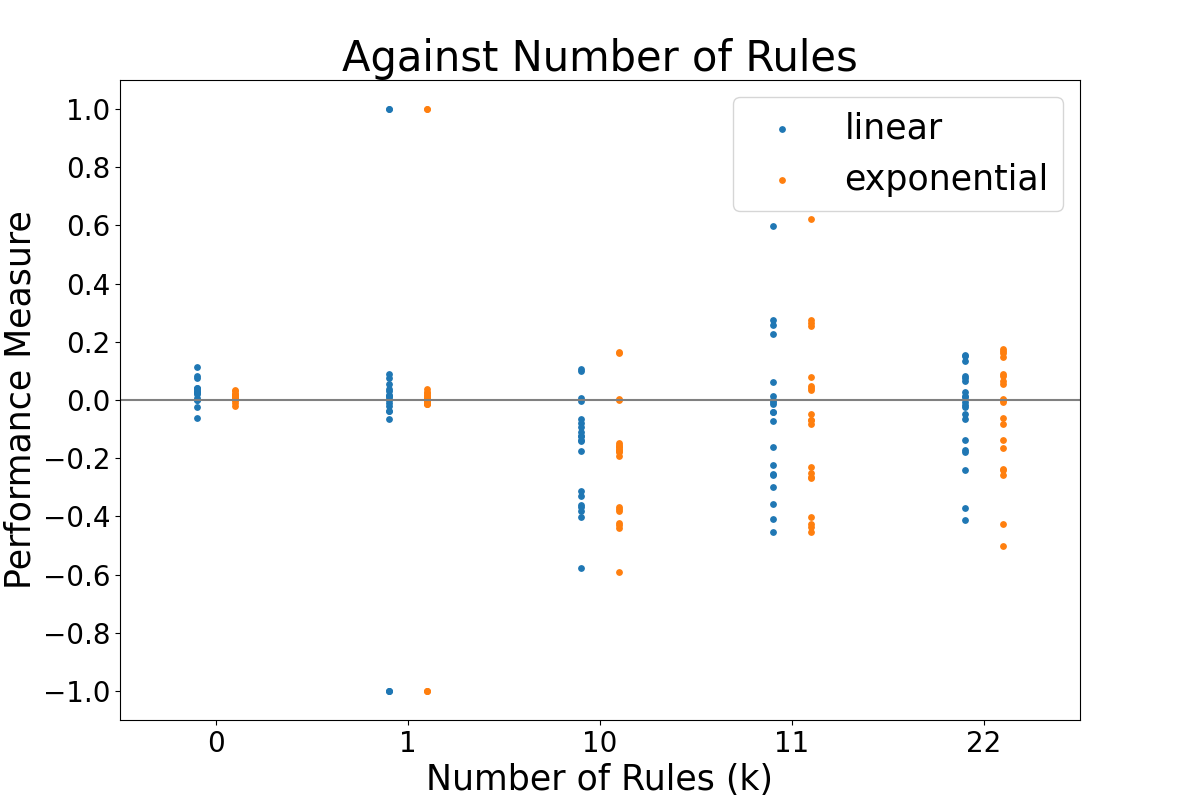
\includegraphics[width = \textwidth]{images/rules_performance_meas.png}
\end{subfigure}
\hfill
\begin{subfigure}{0.49\textwidth}
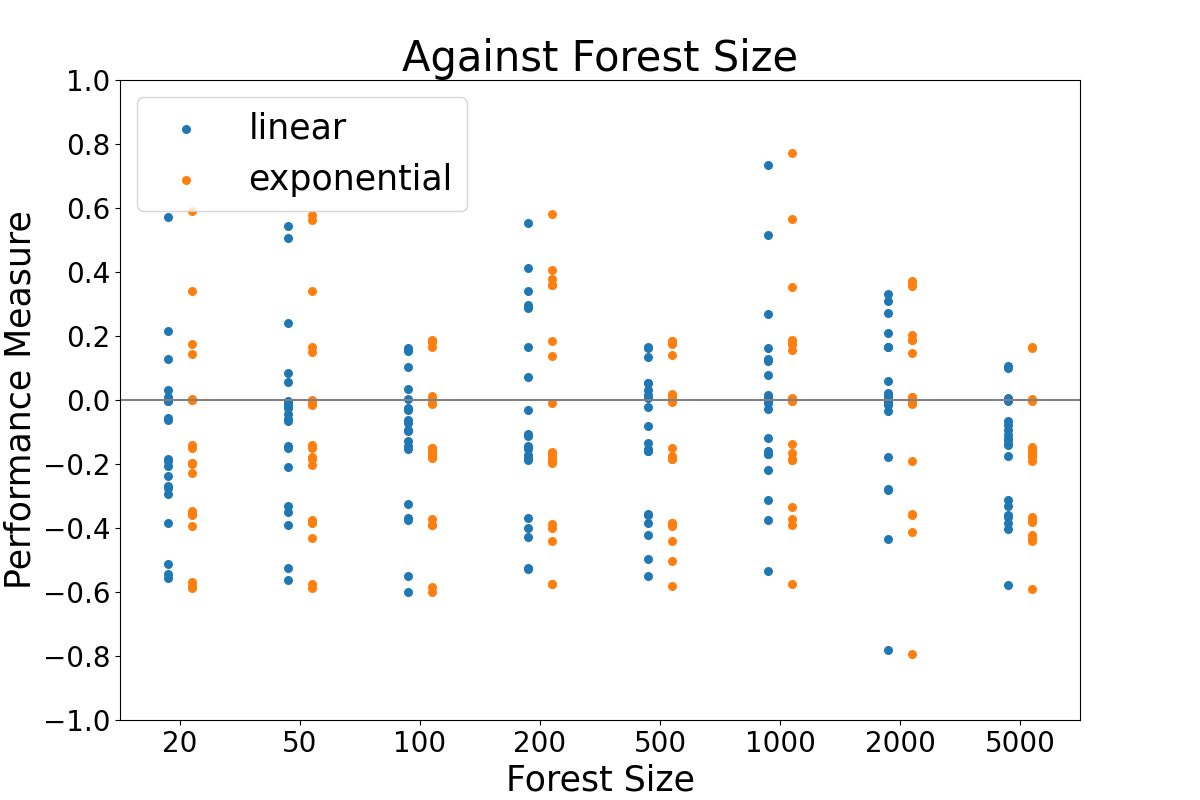
\includegraphics[width = \textwidth]{images/forest_performance_meas.png}
\end{subfigure}
\caption{The performance metric, according to equation~\ref{eq:rule_meas}, for the Tic-tac-toe data set. The number of rules and forest size are shown here using a linear weight function (blue/left) and the exponential weight function (orange/right). It can be seen that the performance is stochastic around a small negative value.}
\label{fig:quant_stat}
\end{figure}

%---------------------------------------------------------------------

\section{Discussion}
\label{sec:dis}
We discuss our contributions and possible future work. Furthermore, we talk about rules as an interpretation aid. 
\subsection{Contributions and Future Work}
As can be seen from the experimental results, the general pattern of the algorithm was not optimistic. Nevertheless, the algorithm developed was able to pull out some general patterns, especially when patterns were searched for from multiple runs. Furthermore, there was an evidential difference in the rules deduced from better forests, meaning there is a relationship between the quality of the forest structure and the quality of the rules deduced. The algorithm would likely be improved if a couple of crucial facets were addressed:
\begin{enumerate}
\item better statistical analysis of how to construct the covariance matrix and how to weight rules, rule elements, and classes according to eigendecomposition characteristics, 
\item expansion of the algorithm to deal with intervals from ordinal and real-valued features,
\item more sophisticated analysis of the quantitative measure function in equation~\ref{eq:rule_meas}, and
\item expansion of the algorithm to consider relationships between rules from the same tree before adding them to the covariance matrix. 
\end{enumerate}
Since this algorithm did not successfully tackle any of these points, it serves as the starting point for a larger project that could build off the concept outlined here. 

\subsection{Rules as an Interpretation Aid}
Many issues stemmed from not correctly understanding how to use logical rules as an interpretation aid. As discussed in the related works, preexisting methods use rules to understand structures like neural networks. In development, most of the focus was on forest-specific literature and other methods that address representing either trees or forests. To improve this method, guidance should be taken from those related works to address better how to present the ruleset. For example, in theory, giving the counterfactuals of ordinal data points seemed logical, but in testing, it added little understanding to the logical rule. The fundamental algorithm might perform better if the rules were displayed with a more rigorously backed measure function. 

%---------------------------------------------------------------------

\section{Conclusion}
\label{sec:conc}
This paper presented a new approach to compiling information over a random forest and attempted to extract rule sets directly from the derived covariance matrix. These rules were implied from eigenvalues of the covariance matrix and would hypothetically result in rules characterized by positive clauses, negative clauses, and an implication of one or more classes. Because of the interconnected nature of the rules, a new performance metric was derived. In empirical testing, the added understandability from the logical rule sets seemed flawed. It motivated a new approach to representing these rule sets and extracting understandable patterns from the forests. It seemed that either insufficient rigor was spent deriving the rules, or the proposed metric was flawed. This work is a good motivator for future work based on the same theory. The next steps include a more complete survey of the current state of rule representation of ILP models and representative models of neural networks. 

At the beginning of the paper, it was stated that the fundamental purpose of the work was to develop a better understanding of the topics of random forests, logical rule sets, and general machine learning practices. In this pursuit, the project was an undeniable success. By developing an algorithm that appears to have failed in its initial aim, we have gained an understanding of what works and the amount of rigor that needs to go into an algorithm's base to cultivate success. This project will continue to be developed in the authors' free time to hopefully derive a visualization technique in line with the original motivation. 


%---------------------------------------------------------------------

\vskip 0.2in
\bibliography{random_forest_rule_extraction}

\end{document}

